\chapter{Введение}
Это руководство сопровождает выпуск версии 2.1.0 Open Source Field Operation And Manipulation (OpenFOAM) 
(операции и манипуляции с полями с открытым исходным кодом) C++ библиотек. Оно предоставляет описание основных операций
 с OpenFOAM, сначала посредством ряда примеров руководства в главе 2 и далее с использованием более детальных описаний 
индивидуальных компонент, которые составляют пакет OpenFOAM.
OpenFOAM это во-первых и прежде всего \textit{библиотеки на C++}, использованные сначала для создания исполняемых модулей 
(executables), называемых как \textit{приложения} (\textit{applications}). Приложения разделяются на две категории:
 решатели или \textit{солверы} (\textit{solvers}), каждый из которых создан чтобы решить частную задачу в механике сплошной
 среды; и сервисные программы или \textit{утилиты} (\textit{utilities}), которые разрабатывались для выполнения задач
 включающих обработку данных.  Дистрибутив OpenFOAM содержит многочисленные решатели и утилиты обеспечивающие
 решение широкого диапазона задач, как описано в главе 3.
Одна из наиболее сильных возможностей OpenFOAM заключается в том, что новые решатели и утилиты могут быть созданы его
 пользователями с некоторыми предварительными, минимально необходимыми знаниями основных использованных методов физики
 и методов программирования.
OpenFOAM поставляется с вычислительной средой включающей  пре- и постпроцессор. Интерфейс (связь с) пре- и постпроцессором
 обеспечивается утилитами OpenFOAM, таким образом гарантируя совместимость обращения с данными для всей вычислительной среды.
 Общая структура OpenFOAM показана на Рис 1.1. ( Figure 1.1.) Обработка предпроцессором и запуск кейса
OpenFOAM представлен в главе 4.
\begin{figure}[h]
 \centering
 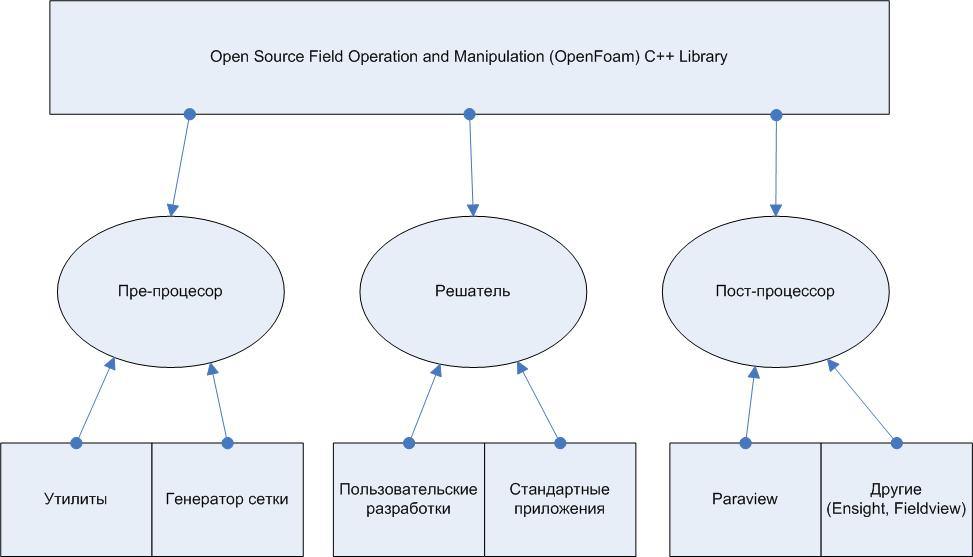
\includegraphics[width=531pt,height=273pt]{UGFigure1-1.PNG}
 % UGFigure 1-1.PNG: 973x557 pixel, 96dpi, 25.74x14.74 cm, bb=0 0 730 418
 \label{fig:1.1}
 \caption{Рисунок 1.1: Условная структура пакета}
\end{figure}

 В главе 5 мы представили как  генерацию (создание) сеток, используя  утилиты генерации сеток
 поставляемых с OpenFOAM, так и преобразование сеточных данных, созданных c использованием сторонних продуктов.
 Постпроцессорная обработка решения описана в 6 главе.